% Created 2024-07-08 Mon 22:16
% Intended LaTeX compiler: pdflatex
\documentclass[15pt]{article}
\usepackage[utf8]{inputenc}
\usepackage[T1]{fontenc}
\usepackage{ragged2e}
\usepackage{caladea}
\usepackage{graphicx}
\usepackage{longtable}
\usepackage{wrapfig}
\usepackage{rotating}
\usepackage{epigraph}
\usepackage[normalem]{ulem}
\usepackage{hyperref}
\usepackage{amsmath}
\usepackage{amssymb}
\usepackage{capt-of}
\usepackage{hyperref}
\usepackage{fancyhdr}
\title{Novena à Santa Bibiana}
 % \hypersetup{
 %  pdfauthor={},
 %  pdftitle={Novena a/à SANTO_NOME},
 %  pdfkeywords={},
 %  pdfsubject={},
 %  pdfcreator={Emacs 29.4 (Org mode 9.6.15)}, 
 %  pdflang={English}
 % }

\title{
  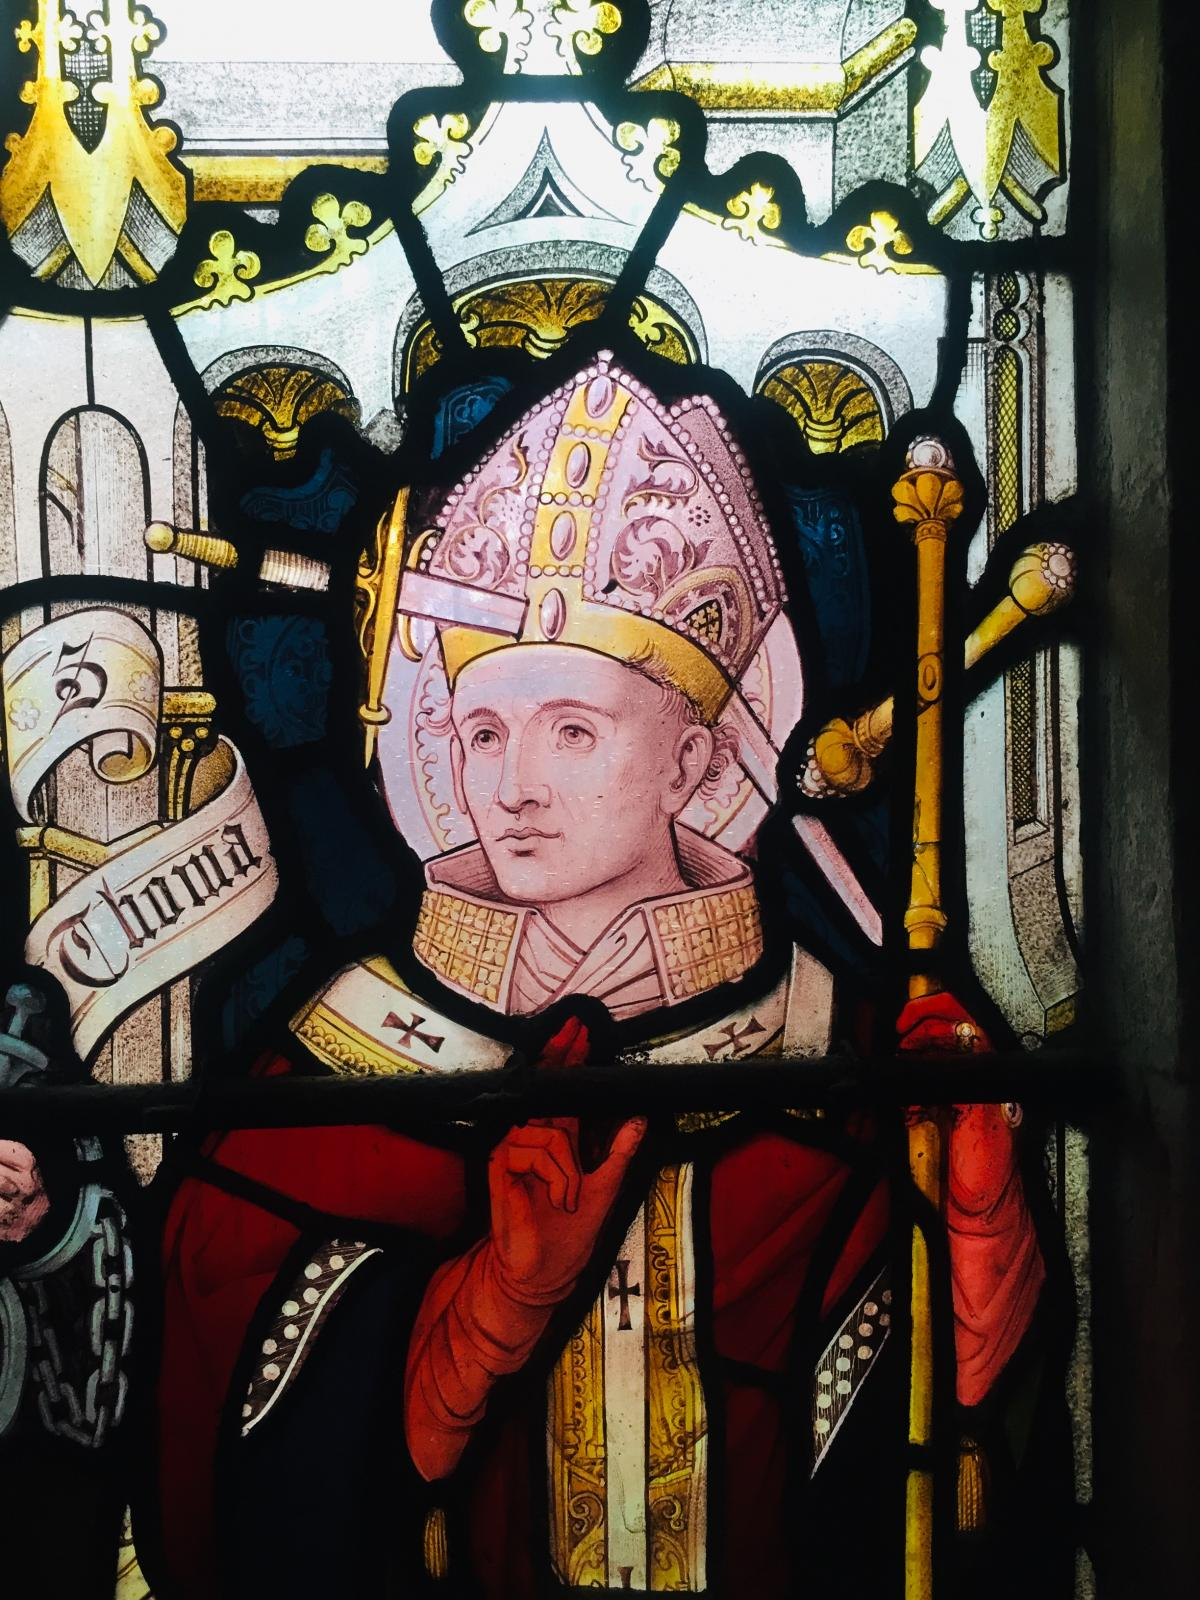
\includegraphics[scale=0.35]{./assets/imagem.jpg}
  \par
   NOVENA A SAO TOMÁS BECKET}
\author{Garamog, Nina Freitas}
\date{20/12 - 29/12}
\renewcommand{\contentsname}{Sumário}

\begin{document}
\maketitle

\thispagestyle{empty}


\pagestyle{fancy}
\fancyhf{} % clear existing header/footer entries
\fancyfoot[LO, CE]{
  
\includegraphics[scale=0.2]{./assets/cross.png} São Tomás Becket, rogai por nós!
}
% Place Page X of Y on the right-hand
% side of the footer
\fancyfoot[R]{\thepage}


  
\newpage

\tableofcontents

\centering
\vfill
Visite-nos no Telegram: \url{https://t.me/CotidieNovena}
\newpage




\begin{justify}

\begin{center}
 \section{História}
\end{center}

\subsection{Origens}\label{sub:Origens} % (fold)

% subsection Origens (end)
São Tomás Becket nasceu no ano 1118 em Londres. Sua família era oriunda da Normandia. Desde muito novo, foi enviado à carreira eclesiástica. Formou-se na Abadia de Merton e, logo em seguida, frequentou a universidade de Bolonha, destacando-se pelas qualidades intelectuais.

\subsection{Chanceler}\label{sub:} % (fold)

Em 1154, Henrique II, rei da Inglaterra e de parte da França, nomeou Tomás Becket como seu chanceler. Homem de confiança do rei, vivia uma vida de bem-estar e não renunciava às insígnias e aos privilégios do poder. Apesar de estar diante do soberano, São Tomás Becket jamais deixou de ser generoso com os mais necessitados.

\subsection{A Ordenação e uma nova vida}\label{sub:} % (fold)

A mudança na vida de São Tomás Becket aconteceu, em 1162, após ser ordenado sacerdote e sagrado Bispo dois dias depois. A partir disso, tornou-se a pessoa mais irrelevante a seguir ao rei. Tomás mudou inteiramente de vida, convertendo-se num dos prelados mais austeros.
São Tomás Becket: separou os deveres políticos da vida religiosa 

\subsection{O Pedido de Demissão}\label{sub:} % (fold)

Convencido de que o cargo de primeiro-ministro e o de príncipe da Inglaterra eram incompatíveis, Tomás pediu demissão do cargo de chanceler, o que descontentou muito o rei. 

\subsection{A Perseguição}\label{sub:} % (fold)

Henrique II ficou ainda mais aborrecido quando, em 1164, por ocasião dos “concílios” de Clarendon e Northampton, o Arcebispo tomou o partido do Papa contra ele. Tomás viu-se obrigado a fugir, disfarçado de irmão leigo, e foi procurar asilo em Compiègne, junto de Luís VII. Passou, a seguir, à abadia de Pontigny e depois à de Santa Comba, na região de Sens.
O Regresso à Pátria e o Sofrimento

\subsection{Inglaterra}\label{sub:} % (fold)

Decorridos quatro anos, a pedido do Papa e do rei da França, Henrique II acabou por consentir que Tomás regressasse à Inglaterra. Persuadiu-se de que poderia contar, daí em diante, com a submissão cega do Arcebispo, mas em breve reconheceu que muito se tinha enganado, pois este continuava a defender as prerrogativas da Igreja romana contra as pretensões régias.

\subsection{Páscoa}\label{sub:} % (fold)

Desesperado, o rei exclamou um dia: “Malditos sejam os que vivem do meu pão e não me livram deste padre insolente”. Quatro cavaleiros tomaram à letra estas palavras, que não eram sem dúvida mais que uma exclamação de desespero. A 29 de dezembro de 1170, à tarde, vieram encontrar-se com Tomás no seu palácio, exigindo que ele levantasse as censuras que tinha imposto. Recusou-se a isso e foi com eles tranquilamente para uma capela lateral da Sé. “Morro de boa vontade por Jesus e pela santa Igreja”, disse-lhes; e eles abateram-no com as espadas.

\subsection{Via de Santificação}\label{sub:} % (fold)

O assassinato de São Tomás Becket comoveu muitos, tanto que, após três anos, no dia 21 de fevereiro de 1173, o Papa Alexandre III sancionou o seu martírio, elevando-o à honra dos altares.

\end{justify}

\subsection*{Créditos:}
\href{https://santo.cancaonova.com/santo/sao-tomas-becket-defensor-da-justica-e-da-igreja/}{Canção Nova}

\newpage

%%%%%%%%%%%%%%%%%%%%%%%%%%%%%%%%%%%%% Orações  %%%%%%%%%%%%%%%%%%%%%%%%%%%%%%%%%%%%%%%%%%%

\section{Orações}\label{sec:Orações} % (fold)
\subsection{Oração Inicial}\label{subsec:OraçãoInicial} % (fold)

Grande Santo, Bispo, Padre, Mártir, e cordeiro sacrificial pela fé, rogai por nós.

Vós, que fostes um Pastor destemido do povo de Deus, rogai por nós para que tenhamos a coragem em todas as circunstâncias de nossas vidas, para vivermos de acordo com a Luz que o vosso exemplo dá às nossas consciências.


Que sejamos fiéis até a morte, como fostes. Que possamos sempre buscar os santos desígnios de Deus em nossas vidas.


São Tomás, muitos foram trazidos a você para cura tanto em sua vida quanto especialmente após seu martírio, por favor, ouça e aceite minhas orações por \emph{(mencione seu pedido aqui…)}


Confiamos que agora, vós, que estais diante do Trono SAgrado de Deus, intercedereis por nós e nos aproximareis de Cristo.

São Tomás, rogai por nós, para que nele, e com ele, possamos viver, nos mover e existir.

\subsection{Oração Final}\label{subsec:OraçãoFinal} % (fold)

\textbf{Pai Nosso, Ave Maria, Glória ao Pai.}

\subsection*{Créditos:}
\href{https://catholicnovenaapp.com/novenas/st-thomas-becket-novena/}{Catholic Novena App}


\end{document}
